The natural method of transmitting electricity from point A to point B is to simply use a conducting wire to connect the two points. However when this simple wire is exposed to the realities for the world, outside effects (eg. magnetic) being to become significant, especially if there are two electrical lines withing close proximity, which often can occur when transmitting a signal to and from a location. These effects can be minimized by using a twisted pair of cables, but at high frequencies there will be significant losses due to radiation into the world or other electrical components. \cite{feynman}

\\
The solution to this problem is to "shield" the cables by wrapping the cable in a conductive material. This creates a Faraday cage against external magnetic fields. This shielding in coaxial cables is combined with a precisely sized dielectric material to control its electrical properties.

\\
Hence we now have the coaxial cable modelled as an inner wire surrounded by a conductive tube at a regulated distance away. Hence modelling it as two conducting cylinders is appropriate as is shown in Figure \ref{fig:coax_theory_1}. We then decide to denote the two conductors as parallel wires if we take a look at them along the wire's axis, as represented in Figure \ref{fig:coax_theory_2}. 

\\
\begin{figure}[h]
\centering
\begin{subfigure}{.5\textwidth}
  \centering
  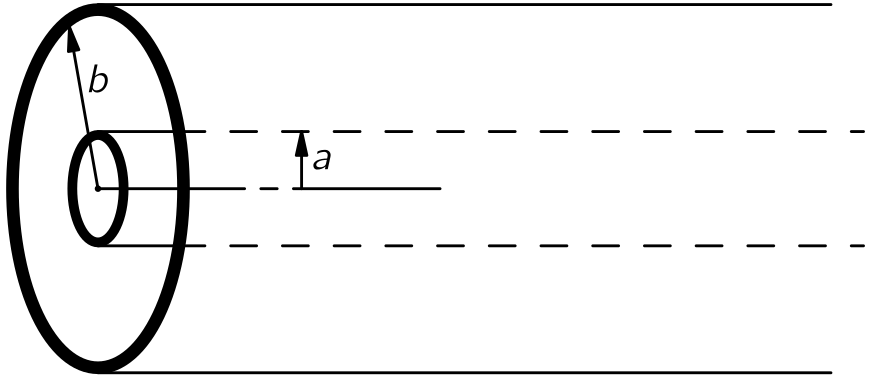
\includegraphics[width=.666\linewidth]{figures/coaxial_derivation_1.png}
  \caption{A coaxial transmission line. \cite{feynman}}
  \label{fig:coax_theory_1}
\end{subfigure}%
\begin{subfigure}{.5\textwidth}
  \centering
  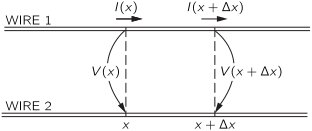
\includegraphics[width=.75\linewidth]{figures/coaxial_derivation_2.png}
  \caption{A coaxial transmission line along its radial axis \cite{feynman}}
  \label{fig:coax_theory_2}
\end{subfigure}
\caption{The coaxial cable representations}
\label{fig:test}
\end{figure}


We then note that we can denote the two currents and voltages separated at points $x$ and $ x + \Delta x$ are (as seen in Figure \ref{fig:coax_theory_2} ). Noting that in an AC circuit $V(t) = L \frac{di(t)}{dt}$ Therefore we can write that:

\begin{align*}
    V(x) + \Delta V &= V( x + \Delta x) \\
            \Delta V &= V( x + \Delta x) - V(x)\\
            \Delta V &= -L \Delta x \frac{di}{dt}\\
\shortintertext{Taking, $\Delta x \rightarrow 0$. Lets us state:}\\
\frac{\partial V}{\partial x} &= -L \frac{di}{dt} \numberthis \label{VtoI}\\
\end{align*}
\\

Which lets us state that the changing current gives us the gradient of voltage with a proportionality relative to the Inductance ($L$).
\\
Next we can also take a look at the capacitance between the two wires, which in lets us state that between $x$ and $ x + \Delta x$  is a charge q which follow the relationship:\\

\begin{align*}
   q &= \frac{q}{V} V \Delta x \\
   q &= C V \Delta x \\
\shortintertext{Therefore with respect to time it is:}\\
\Delta I &= C \Delta x \frac{\partial V}{\partial x} \\
\shortintertext{Taking, $\Delta x \rightarrow 0$ Lets us state:}\\
\frac{\partial I}{\partial x} & -C \frac{dv}{dt} \numberthis \label{ItoV}\\
\end{align*}

Then we can combine these two equations (which are the basic equations of a transmission line) to obtain:

\begin{align*}
    \frac{\partial^2 V}{\partial x^2} &= C L \frac{\partial^2 V}{\partial t^2} \numberthis \label{V2}\\ % Not to be confused with the residence this is V to the 2
\shortintertext{Or we can obtain:}\\
    \frac{\partial^2 I}{\partial x^2} &= C L \frac{\partial^2 I}{\partial t^2} \numberthis 
    \label{I2}\\
\end{align*}

We can then see that clearly the wave equation will solve this equation which means that:

\begin{align*}
    V &= V_1 e^{i(\omega t - kx)} + V_2 e^{i(\omega t + kx)} \numberthis \label{v_wave}\\
    I &= I_1 e^{i(\omega t - kx)} + I_2 e^{i(\omega t + kx)} \numberthis \label{i_wave}\\
\end{align*}

Therefore by inputting Equation \ref{v_wave} into Equation \ref{V2} or Equation \ref{i_wave} into \ref{I2} we can obtain the fact that:
\begin{align*}
    \left( \frac{k}{\omega} \right) ^2 &= L C
\shortintertext{Which means that:}\\
\abs*{ \frac{\omega}{k} }&= \frac{1}{\sqrt{L C}} \numberthis \label{LCconvert}
\shortintertext{But noting that we know wave velocity $v$ $ = \frac{\omega}{k}$}\\
    v = \frac{\omega}{k} &= \pm \frac{1}{\sqrt{L C}} \numberthis \label{velocity}
\end{align*}

We now can take the wave equations \ref{v_wave} \& \ref{i_wave} and reinsert them into our original relations of $I$ to $V$ in Equations \ref{VtoI} \& \ref{ItoV}. Doing this lets us state:

\begin{align*}
\shortintertext{First we will insert \ref{v_wave} \& \ref{i_wave} into \ref{VtoI} : }
    \frac{\partial}{\partial x} \left( V_1 e^{i(\omega t - kx)} + V_2 e^{i(\omega t + kx)} \right) &= -L \frac{\partial}{\partial t} \left( I_1 e^{i(\omega t - kx)} + I_2 e^{i(\omega t + kx)} \right)\\
    ik \left( - V_1 e^{i(\omega t - kx)} + V_2 e^{i(\omega t + kx)} \right) &= -L i \omega \left( I_1 e^{i(\omega t - kx)} + I_2 e^{i(\omega t + kx} \right)\\
    +\frac{k}{\omega} V_1 e^{i(\omega t - kx)} - \frac{k}{\omega} V_2 e^{i(\omega t + kx)} &= L \left( I_1 e^{i(\omega t - kx)} + I_2 e^{i(\omega t + kx)} \right)\\
\shortintertext{But noting that $\pm \frac{k}{\omega} = \sqrt{ L C } $ can let us say:}\\
    \sqrt{ L C } \left( V_1 e^{i(\omega t - kx)} + V_2 e^{i(\omega t + kx)} \right) &= L \left( I_1 e^{i(\omega t - kx)} + I_2 e^{i(\omega t + kx)} \right)\\
    V  &= \frac{L}{\sqrt{ L C}} I \\
\shortintertext{And by definition, the impedance $Z = \frac{V}{I}$:}\\
\Aboxed{   Z_o = \frac{V}{I} &=  \sqrt{\frac{L}{C}} }\\  \numberthis \label{charcteristic_impedance}
\end{align*}

This quantity $Z_o$ is known as the characteristic impedance, which means that the cable acts with an impedance of $Z_o$ if it is of infinite length. We note if characteristic impedance was to be matched by a resistor at the end of the cable, then it would absorb all of the power which hit it. This means the finite length cable would act as if it was infinite. This type of  cable termination is called \textbf{matched} and will not reflect any signals at cable termination.

\\

We can also look at two other types of cable terminations. The first case is if the cable has nothing at the end of the cable. This is known as \textbf{open} and means that the current will be 0 by definition (it will be a node) and the voltage will be maximal (anti-node). We will denote the end of the cable as $x_{end}$. This means we can re-write the wave equation with these boundary equations, stating with current:

\begin{align*}
    I_{end} = 0 &=  I_1 e^{i(\omega t - kx)} + I_2 e^{i(\omega t + kx)} \\
\shortintertext{But we note that the wave is simply being reflected off of the end of the cable which means $I_1 = I_2 = I_o$. But $I_o$ is only an amplitude so we will define the wave as:} \\
     0 &= I_o ( \pm e^{i(\omega t - kx_{end})} \pm e^{i(\omega t + kx_{end}})) \\
     0 &= I_o e^{i\omega t} (\pm e^{-i kx_{end}} \pm e^{+i kx_{end}}) \\
     0 &= I_o (\pm e^{-i kx_{end}} \pm e^{+i kx_{end}})\\ \numberthis \label{signed_I}
\shortintertext{Noting $sin(0)$ = $0$ we can then note the solution of:}
    0 &= I_o (e^{-i kx_{end}} - e^{+i kx_{end}})
\shortintertext{Which means that the general solution is:}
\Aboxed{    I &= I_o (e^{i(\omega t - k(x - x_{end}))} - e^{i(\omega t + k(x - x_{end}))}) }\\
\shortintertext{Similarly by noting the solution of cos(0) = 1 and changing the signage at equation \ref{signed_I} appropriately we can state:}\\
\Aboxed{    V &= V_o (e^{i(\omega t - k(x - x_{end}))} + e^{i(\omega t + k(x - x_{end}))}) }\\
\end{align*}

We also wish to see what the impedance will look like at x = 0, which will give us:

\begin{align*}
    Z_{in} &= \dfrac{V_o (e^{i(\omega t - k(0 - x_{end}))} + e^{i(\omega t + k(0 - x_{end}))})}{I_o (e^{i(\omega t - k(0 - x_{end}))} - e^{i(\omega t + k(0 - x_{end}))})}\\
         &= Z_o \dfrac{ e^{i(\omega t)} e^{-i kx_{end}} - e^{+i kx_{end}} } { e^{i(\omega t)} e^{-i kx_{end}} + e^{+i kx_{end}}}\\
         &= Z_o \dfrac{2 cos(kx_{end})}{ 2i sin (kx_{end})}\\
         &= -i Z_o \dfrac{cos(kx_{end})}{sin (kx_{end})}\\
\Aboxed{    Z_{in} &= -i Z_o cot(kx_{end})}\\ \numberthis \label{Zin_open}
\end{align*}

We then look at the final case where there is a bridge made at the end of the cable, or it is \textbf{shorted}. This means that current will be maximal (it will be an anti-node) and the voltage will be 0 (node). We can represent these waves as the opposite of the open cables stating with equation \ref{signed_I} and building to get:


\begin{align*}
 \Aboxed{   I &= I_o (e^{i(\omega t - k(x - x_{end}))} + e^{i(\omega t + k(x - x_{end}))}) }\\
 \Aboxed{   V &= V_o (e^{i(\omega t - k(x - x_{end}))} - e^{i(\omega t + k(x - x_{end}))}) }\\
\shortintertext{Following a similar procedure as we saw in the open cable:}
    Z_{in} &= Z_o \dfrac{ 2i sin (kx_{end})}{2 cos(kx_{end})}\\
\Aboxed{    Z_{in} &= i Z_o tan(kx_{end})}\\ \numberthis \label{Zin_short}
\end{align*}

We will note that during this derivation we have assumed a lossless cable, hence in real situations we will get systematic losses known as attenuation of the signal.

Finally we will take a look again at Figure \ref{fig:coax_theory_1}. Our goal here is to calculate values of C and L. Regarding the cylindrical shell of thickness $dr$ and length $\elll$ we are able to state that energy (U) is:

\begin{align*}
\shortintertext{After noting that the magnetic energy will be an integral of $\left. \epsilon_o c^2 B^2 \middle/ 2 \right.$:}
    U &= \int_{a}^{b} r \; dr \; \int_{0}^{\theta} d \theta \int_{0}^{\ell} dz \; \frac{\epsilon_o c^2 B^2}{2} \\ 
      &= \int_{a}^{b} r \; dr \; 2 \pi \frac{\epsilon_o c^2 B^2}{2} \\
\shortintertext{Noting that $B = \frac{I}{2 \pi \epsilon_o c^2 r}$ for a cylindrical conductor:}
    U &= \epsilon_o c^2 \frac{1}{2} \int_{a}^{b} \; dr \; \ell \left( \frac{I}{2 \pi \epsilon_o c^2 r }\right) ^2  \ell 2 \pi r \\
      &= \frac{1}{2} \int_{a}^{b} \; dr \; \frac{I^2 \ell}{2 \pi \epsilon_o c^2 r } \\
      &= \frac{I^2 \ell}{4 \pi \epsilon_o c^2} \int_{a}^{b} \frac{dr}{r} \\
    U &= \frac{I^2 \ell}{4 \pi \epsilon_o c^2} \; ln \left( \frac{b}{a} \right)\\
\shortintertext{Noting that the energy stored in an inductor is defined as $U = \frac{1}{2} L I^2$ and noting $\epsilon_r$ for permitivity of a non-vacuum:}
 \Aboxed{   L &= \frac{\ell \; ln \left( b \middle/ a \right) }{2 \pi \epsilon_o \epsilon_r c^2}} \numberthis \label{inductance}
\shortintertext{Noting the velocity of electricity in a vacuum is c by definition and using equation \ref{velocity} gives us:}
    c &= \frac{1}{\sqrt{L C}}  \\
    \frac{1}{c^2} &= \frac{\ell \; \; ln \left( b \middle/ a \right) }{2 \pi \epsilon_o \epsilon_r c^2} C \\
\Aboxed{    C &= \frac{\ell \; 2 \pi \epsilon_o }{ln \left( b \middle/ a \right) }} \numberthis \label{conductance} \\
\shortintertext{Therefore by using the calculated values of L and C in equation \ref{charcteristic_impedance} we get:}
\Aboxed{    Z &= \frac{\ell \; ln \left( b \middle/ a \right) }{2 \pi \epsilon_o \epsilon_r \; c }} \numberthis \label{impedance} \\
\end{align*}

